\documentclass[%
	paper=a4,
	fontsize=10pt,
	DIV11,BCOR10mm,
	numbers=noenddot,
	abstract=yes
]{scrartcl}

\usepackage[utf8]{inputenc}
\usepackage[english]{babel}
\usepackage[T1]{fontenc}
\usepackage{tgpagella}
\usepackage{microtype}


\usepackage{textcomp}
\usepackage{gensymb}


\usepackage{graphicx}
\graphicspath{{figures/}}


\usepackage{xfrac}
\usepackage{units}


\usepackage{booktabs}


\usepackage{amsmath}
\usepackage{amssymb}
\usepackage{amsthm}


\usepackage{mathtools}
\mathtoolsset{showonlyrefs=true}


\usepackage{scrhack} % for algorithm package
\usepackage[boxed]{algorithm}
\usepackage{algpseudocode}


\usepackage[
	style=alphabetic,
	bibstyle=alphabetic,
	maxbibnames=100,
	giveninits=true,
	useprefix=true,
	natbib=true,
	backend=biber]{biblatex}
\usepackage[strict=true]{csquotes}
\addbibresource{references.bib}


\usepackage{hyperref}
\hypersetup{
	%colorlinks,
	%citecolor=black,
	%filecolor=black,
	%linkcolor=black,
	%urlcolor=black,
	pdfauthor={Christoph Conrads},
	unicode=true,
}


% Make links jump to the beginning of figures and tables, not to the caption in
% them.
% This can also be fixed with the caption package.
\usepackage[all]{hypcap}



% bibliography with ngerman: @mastersthesis != Magisterarbeit
\DefineBibliographyStrings{english}{%
	mathesis = {MSc thesis},
}
\DefineBibliographyStrings{ngerman}{%
	mathesis = {Masterarbeit},
}



% Command definitions
\newcommand{\bigOh}[1]{\mathcal{O}(#1)}
\newcommand{\cond}[2][]{\kappa_{#1}(#2)}
\newcommand{\function}[1]{\textsc{#1}}
\newcommand{\almost}[1]{\widetilde{#1}}
\newcommand{\set}[1]{\mathcal{#1}}

\newcommand{\R}{\mathbb{R}}
\newcommand{\F}{\mathbb{C}}

\newcommand{\macheps}{\varepsilon}
\newcommand{\unitRO}{\mathbf{u}}
\newcommand{\tol}{\operatorname{tol}}

\DeclarePairedDelimiter\abs{\lvert}{\rvert}
\DeclarePairedDelimiter\norm{\lVert}{\rVert}
\DeclarePairedDelimiter\ceil{\lceil}{\rceil}

\DeclareMathOperator{\diag}{diag}
\DeclareMathOperator{\ran}{ran}
\DeclareMathOperator{\rank}{rank}
\DeclareMathOperator{\mathspan}{span}



\newtheorem{theorem}{Theorem}[section]
\newtheorem{corollary}{Corollary}[section]

\theoremstyle{definition}
\newtheorem{example}{Example}[section]
\newtheorem{definition}{Definition}[section]

% \bordermatrix with custom delimiters
% Source: Herbert Voß: "Math mode - v. 2.47", 2014, §5
\makeatletter
\newif\if@borderstar
\def\bordermatrix{\@ifnextchar*{%
    \@borderstartrue\@bordermatrix@i}{\@borderstarfalse\@bordermatrix@i*}%
}
\def\@bordermatrix@i*{\@ifnextchar[{\@bordermatrix@ii}{\@bordermatrix@ii[()]}}
\def\@bordermatrix@ii[#1]#2{%
\begingroup
  \m@th\@tempdima8.75\p@\setbox\z@\vbox{%
    \def\cr{\crcr\noalign{\kern 2\p@\global\let\cr\endline }}%
    \ialign {$##$\hfil\kern 2\p@\kern\@tempdima & \thinspace %
    \hfil $##$\hfil && \quad\hfil $##$\hfil\crcr\omit\strut %
    \hfil\crcr\noalign{\kern -\baselineskip}#2\crcr\omit %
    \strut\cr}}%
  \setbox\tw@\vbox{\unvcopy\z@\global\setbox\@ne\lastbox}%
  \setbox\tw@\hbox{\unhbox\@ne\unskip\global\setbox\@ne\lastbox}%
  \setbox\tw@\hbox{%
    $\kern\wd\@ne\kern -\@tempdima\left\@firstoftwo#1%
      \if@borderstar\kern2pt\else\kern -\wd\@ne\fi%
    \global\setbox\@ne\vbox{\box\@ne\if@borderstar\else\kern 2\p@\fi}%
    \vcenter{\if@borderstar\else\kern -\ht\@ne\fi%
      \unvbox\z@\kern-\if@borderstar2\fi\baselineskip}%
      \if@borderstar\kern-2\@tempdima\kern2\p@\else\,\fi\right\@secondoftwo#1 $%
  }\null \;\vbox{\kern\ht\@ne\box\tw@}%
\endgroup
}
\makeatother

\newcommand{\mybordermatrix}[1]{\bordermatrix[{[]}]{#1}}



\renewcommand{\algorithmicrequire}{\textbf{Input:}}
\renewcommand{\algorithmicensure}{\textbf{Output:}}
\algrenewcommand{\algorithmiccomment}[1]{\hskip1em\# #1}



\newcommand{\propername}[1]{\textsc{#1}}





\title{Polynomial Filtering}
\author{Christoph Conrads {\small \url{https://christoph-conrads.name}}}



\begin{document}

\maketitle

\begin{center}
	\begin{minipage}{0.8\textwidth}
		This work is licensed under the Creative Commons Attribution-ShareAlike
		4.0 International License. To view a copy of this license, visit \\
		\url{http://creativecommons.org/licenses/by-sa/4.0/}
	\end{minipage}

	\vspace{1\baselineskip}

	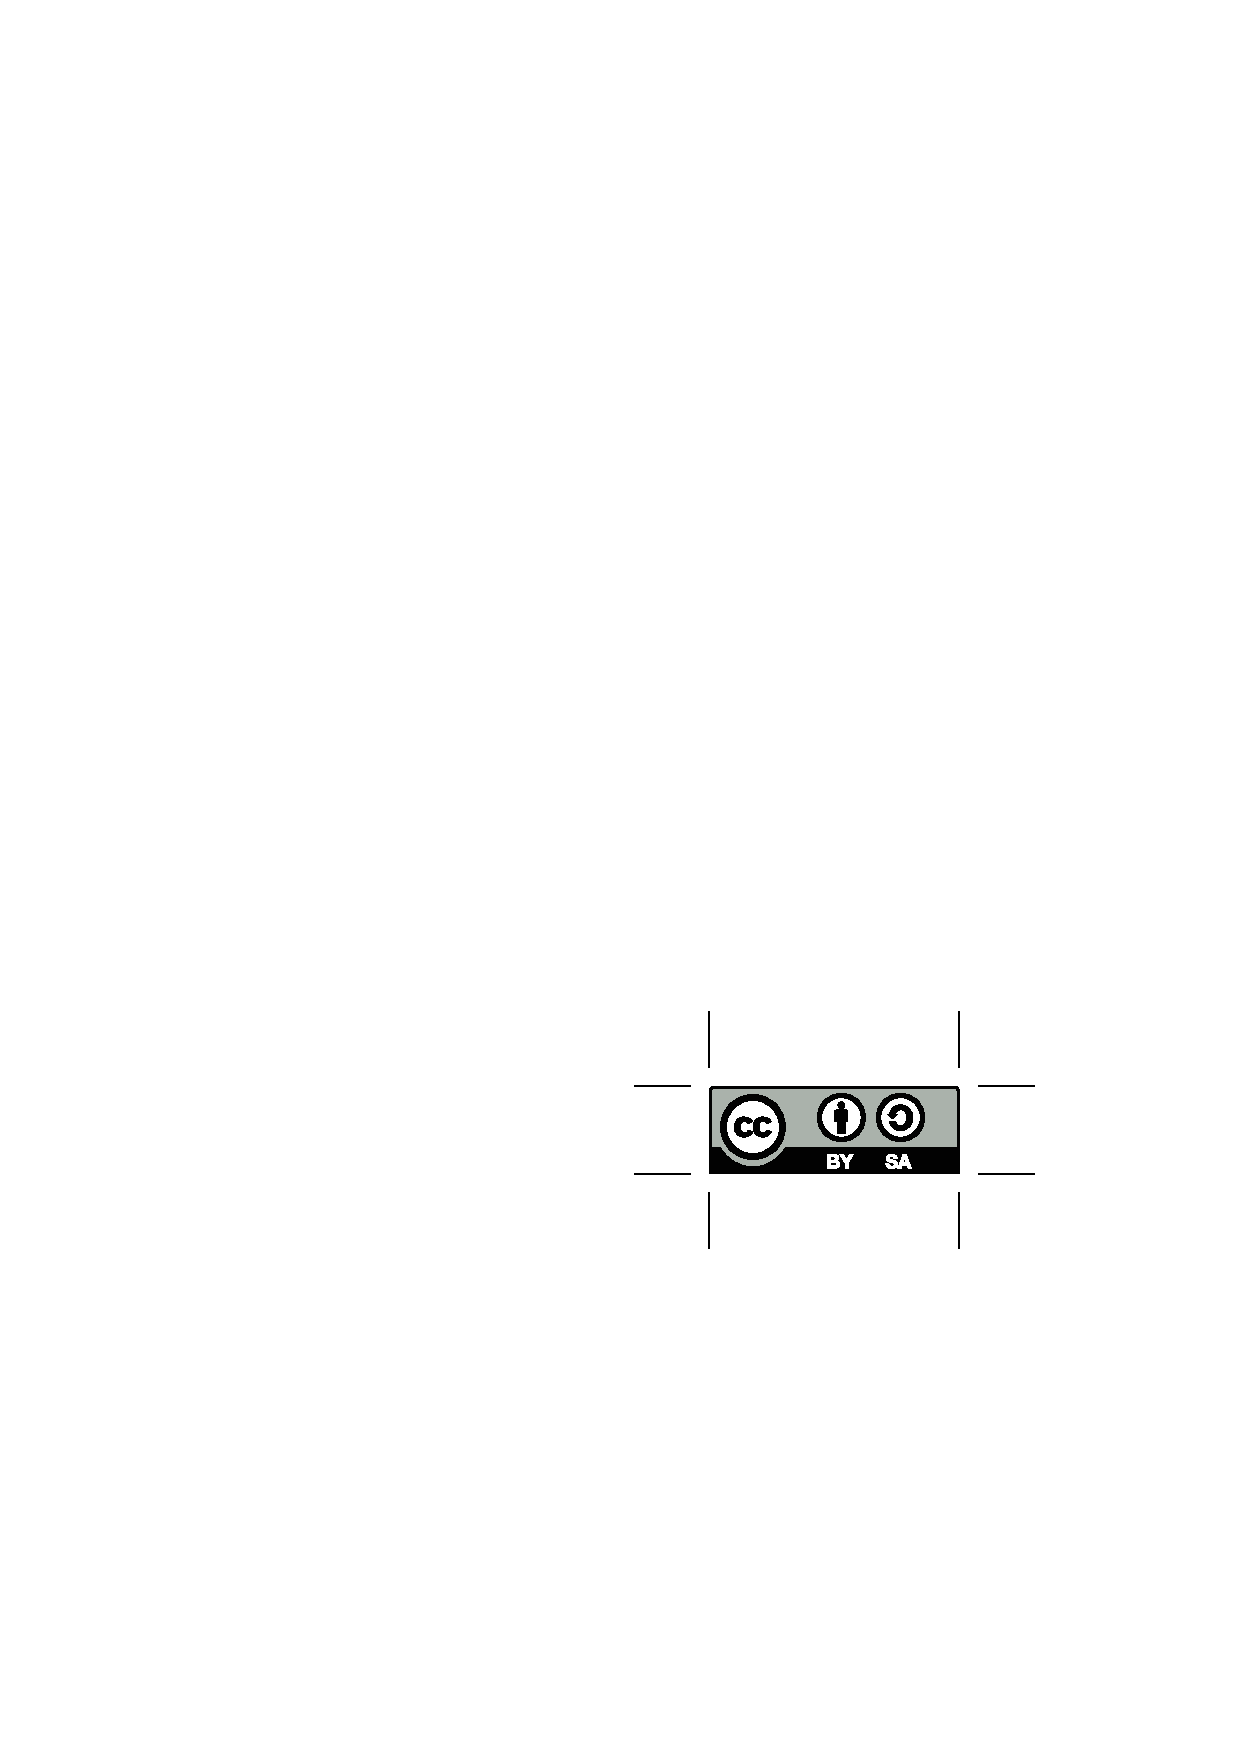
\includegraphics[width=8em]{creative-commons-by-sa}
\end{center}



\section{Motivation}

DCGeig computes all eigenpairs $(\lambda, x)$, of a generalized eigenvalue
problem $Kx = \lambda Mx$, where $\lambda \leq \lambda_c$, $\lambda_c > 0$, $K,
M \in \F^{n,n}$ are Hermitian positive definite (HPD). Assume $K, M$ are
partitioned conformally into $2 \times 2$ block matrices:
\[
	\begin{pmatrix} K_{11} & K_{12} \\ K_{21} & K_{22} \end{pmatrix}
	x
	= \lambda \begin{pmatrix} K_{11} & K_{12} \\ K_{21} & K_{22} \end{pmatrix}x.
\]
Broadly speaking, DCGeig applies the following procedure recursively:
\begin{itemize}
	\item heuristically determine a cutoff value $\lambda_c' > \lambda_c$,
	\item compute all eigenpairs $(\lambda_i, x_i)$ of the subproblems
		$K_{ii} x_i = \lambda_i M_{ii} x_i$, $i = 1, 2$, where
		$\lambda_i \leq \lambda_c'$,
	\item lift $x_i$, $i = 1, 2$, to $F^n$ and use these lifted vectors as
		a search space for the exact eigenvectors of $(K, M)$,
	\item improve the search space,
	\item compute eigenpairs $(\lambda, x)$ of $(K, M)$,
	\item select eigenpairs $\lambda \leq \lambda_c$.
\end{itemize}
The first problem with this approach is the presence of $\lambda_c'$: it cannot
be chosen accurately a priori and if $\lambda_c'$ is too large, then the number
of vectors spanning the search space increases and the solver will be slowed
down or run out of memory; if $\lambda_c'$ is too small, then the search space
for the desired eigenvectors of $(K, M)$ shrinks and the solver will be slowed
down\footnote{Let $s$ be the dimension of the search space and let $\lambda_1
\leq \lambda_2 \leq \dotsb \leq \lambda_n$. The solver uses subspace iterations
[SI] to improve the search space and the convergence rate of SI is directly
related to the ratio $\sfrac{\lambda_c}{\lambda_s}$ - the lower the better
\cite[§5.2]{Saad2011}. Consequently, if $s$ decreases, then
$\sfrac{\lambda_c}{\lambda_s}$ increases.} or miss eigenpairs. The second
problem is the computation of exact (sufficiently accurate) eigenpairs in the
subproblems because what we want to achieve with the recursion is to find a
search space that is large enough to accomodate all desired eigenvectors of $(K,
M)$. Instead, we select the search space based on the eigenvalues $\lambda_i$
and the heuristically selected value $\lambda_c'$.

A faster method yielding a good search space might work as follows:
\begin{itemize}
	\item we compute the number $n_c$ of desired eigenpairs $(\lambda, x)$ of $(K, M)$,
	\item we choose positive integers $n_1$, $n_2$ such that $n_1+n_2 \geq n_c$,
		and
	\item we calculate $n_i$ linearly independent vectors that span the space of
		eigenvectors $x_i$ corresponding to the smallest eigenvalues of
		$(K_{ii}, M_{ii})$, $i = 1, 2$.
\end{itemize}
The question arises, if there are fast methods for the computation (or
estimation) of $n_c$ and we can answer the question in the affirmative. Since
$K$ and $M$ are Hermitian, we can apply Sylvester's law of inertia
\cite[Theorem~4.5.8]{Golub2012}, compute the $LDL^T$ decomposition of $K -
\lambda_c M$, and count the number of non-positive diagonal entries to $D$ to
calculate $n_c$. Algorithms for the sparse $LDL^T$ decomposition are implemented
in MUMPS\footnote{\url{http://mumps.enseeiht.fr/}},
PaStiX\footnote{\url{http://pastix.gforge.inria.fr/}},
SPOOLES\footnote{\url{http://www.netlib.org/linalg/spooles/}},
SPRAL\footnote{\url{http://www.numerical.rl.ac.uk/spral/}}, and
TAUCS\footnote{\url{http://www.tau.ac.il/~stoledo/taucs/}} (SPOOLES and TAUCS are
unmaintained). The major drawback of this approach is the memory consumption due
to the fill-in.

Alternatively, we can use a combination of random sampling and polynomial
filtering to estimate $n_c$ and this approach has been thoroughly analyzed in
\cite{DiNapoli2016}. Rational expansion filtering will not be discussed here
because the author is more familiar with polynomial filtering, because rational
filtering seems to be better suited when it is combined with an iterative solver
(rational filtering requires the factorization of $K - \sigma M$ for different
shifts $\sigma$), and because we would need software for the factorization of
indefinite, Hermitian matrices $K - \sigma M$, i.\,e., we would end up computing
$LDL^T$ decompositions. Rational filtering is already used in practice, e.\,g.,
see \cite{Polizzi2009}.



\section{Estimating Eigenvalue Counts}

Let $A \in \F^{n,n}$ with entries $a_{ij}$, $i,j = 1, 2, \dotsc, n$. Throughout
this text, we assume that $A$ has real eigenvalues.

We need the following theorem about the trace
\[ \operatorname{tr}(A) = \sum_{i=1}^n a_{ii}. \]

\begin{theorem}[{\cite[§2.4.1]{Horn2012}}]
	Let $A \in \F^{n,n}$. Then the trace of $A$ is equal to the sum of its
	eigenvalues:
	\[ \operatorname{tr}(A) = \sum_{i=1}^n \lambda_i. \]
\end{theorem}

The concept of projection will be essential for our purposes.

\begin{definition}[{\cite[§0.9.13]{Horn2012}}]
	Let $P \in \F^{n,n}$. If $P = P^2$, then $P$ is called a \emph{projection}.
\end{definition}

Depending on the literature, $P$ may also be called a \emph{projector}, e.\,g.,
in \cite{Polizzi2009}.

\begin{theorem}
	Let $P \in \F^{n,n}$ be a projection. Then $P$ can only have the eigenvalue
	zero and one.
\end{theorem}

\begin{proof}
	Let $J \in \F^{n,n}$ be the Jordan canonical form of $P$
	\cite[§3.1]{Horn2012}. Since $P = P^2$, it must hold that $J = J^2$ so $J$
	is diagonal. Also, since $J = J^2$, all values on the diagonal of $J$ must
	be one or zero. The diagonal entries of $J$ are the eigenvalues of $P$ and
	this completes the proof (NB: This solves \cite[3.3P3]{Horn2012} partially.)
\end{proof}

The identity matrix is a projection whose spectrum contains only ones whereas
the zero matrix has only the eigenvalue zero. We will now show one way to
construct projections.

\begin{definition}[Isometric Matrix]
	Let $Q \in \F^{n,m}$, $m \leq n$, let $I_m$ be the $m \times m$ identity
	matrix. If $Q^* Q = I_m$, then $Q$ is called \emph{isometric}.
\end{definition}

$Q$ may also be called \emph{Euclidean isometry}
\cite[Definition~2.1.5]{Horn2012}. Note that every column subset of a unitary
matrix forms an isometric matrix.

\begin{theorem}
	Let $Q \in \F^{n,m}$ be isometric. Then $Q Q^*$ is a projection.
\end{theorem}

\begin{proof}
	Let $P = Q Q^*$. It holds that
	\[ P^2 = Q Q^* Q Q^* = Q I_m Q^* = Q Q^* = P. \]
\end{proof}

\begin{theorem}
	Let $Q \in \F^{n,m}$ be isometric. Then the projection $P = Q Q^*$ has the
	eigenvalue one with algebraic multiplicity $m$ and the eigenvalue zero with
	algebraic multiplicity $n - m$.
\end{theorem}

\begin{proof}
	From $Q^* Q = I_m$, it follows that the columns of $Q$ are orthonormal. Let
	$Q = [q_1, q_2, \dotsc, q_m]$ be a column-partitioning of $Q$. Then $P = Q
	Q^*$ can be written as $P = \sum_{i=1}^n q_i q_i^*$. Consequently, $P$ is a
	Hermitian matrix with rank $m$ and eigenvalues one and zero.
\end{proof}

\begin{corollary}
	Let $Q \in \F^{n,m}$ be isometric, let $P = Q Q^*$. Then
	\[ \operatorname{tr}(P) = m. \]
\end{corollary}

Now consider that we want to count the number of eigenvalues of a matrix $A \in
\F^{n,n}$ in the interval~$[a, b]$.

\begin{theorem}[Schur form {\cite[Theorem~2.3.1]{Horn2012}}]
	Let $A \in \F^{n,n}$ have eigenvalues $\lambda_1, \lambda_2, \dotsc,
	\lambda_n$ in any prescribed order. Then there is a unitary matrix $U \in
	\F^{n,n}$ such that $T = U^* A U$ is an upper triangular matrix with
	diagonal entries $t_{ii} = \lambda_i$, $i = 1, 2, \dotsc, n$. If $A$ is real
	and has only real eigenvalues, then $U$ and $T$ can be taken to be real.
\end{theorem}

Let $U = [u_1, u_2, \dotsc, u_n]$ be a column partitioning of $U$. If
$\lambda_1, \lambda_2, \dotsc, \lambda_m$ are all the eigenvalues of $A$ in the
interval~$[a, b]$, then $Q \coloneqq [u_1, u_2, \dotsc, u_m]$ is an isometric
matrix, and $P \coloneqq Q Q^*$ is a projection with trace $m$. Clearly, to
estimate the number of eigenvalues in~$[a, b]$, we can approximate the trace of
$P$.



\section{Approximating An Invariant Subspace Projection}
\label{sec:projection-approximation}

Previously, we showed that we can count the number of eigenvalues in a given
interval~$[a, b]$ of a matrix $A$ by computing the trace of a projection onto
the invariant subspace corresponding to the eigenvalues in~$[a, b]$. In this
section we discuss how we can compute the projection. Obviously, we can
calculate the Schur decomposition of a $A$ to acquire $P$ but when we have the
Schur decomposition, the use of the projection is superfluous. Instead, we can
approximate the projection with polynomials.

Let $h(t): \R \rightarrow \R$ with
\[
	h(t) =
	\begin{dcases*}
		1 & if $t \in [a, b]$, \\
		0 & otherwise.
	\end{dcases*}
\]
If $p(t)$ is polynomial approximation to $h(t)$, then $p(A)$ will be an
approximation to the desired projection $P$. In this article, we will use
Chebyshev polynomials.

\begin{definition}[Chebyshev polynomial]
	The function $T_k: [-1, +1] \rightarrow \R$, where
	\[
		T_k(t) =
		\begin{dcases*}
			0 & if $k = 0$, \\
			t & if $k = 1$, \\
			2 t \, T_{k-1}(t) - T_{k-2}(t) & otherwise,
		\end{dcases*}
	\]
	is called \emph{Chebyshev polynomial} (of the first kind).
\end{definition}

Chebyshev polynomials $T_k(t)$ are orthogonal polynomials and orthogonal
polynomials minimize the mean square error $\int (f(t) - p(t))^2 \,\mathrm{d}t$,
where $f: \R \rightarrow \R$ is a piecewise continuous function and $p: \R
\rightarrow \R$ is an orthogonal polynomial \cite[Chapter II,
§1.3]{Courant1953}.

\begin{theorem}
	It holds that
	\[
		\int\limits_{-1}^{+1} \frac{T_n(t) T_m(t)}{\sqrt{1 - t^2}}\,\mathrm{d}t=
		\begin{dcases*}
			\pi & if $n = m = 0$, \\
			\sfrac{\pi}{2} & if $n = m \neq 0$, \\
			0 & if $n \neq m$.
		\end{dcases*}
	\]
\end{theorem}

Let $d$ be the degree of the polynomial approximating $h(t)$. We can approximate
$h(t)$ with a linear combination of $d$ Chebyshev polynomials such that
\[ h(t) \approx \sum_{k=0}^d \gamma_k T_k(t), \]
where $\gamma_k \in \R$. The coefficients can be computed with the following
expression:
\[
	\gamma_k =
	\int\limits_{-1}^{+1} \frac{h(t) T_k(t)}{\sqrt{1 - t^2}}\,\mathrm{d}t,
	\, k = 0, 1, \dotsc, d.
\]
For the step function $h_{[a,b]}(t)$, the coefficients are \cite{DiNapoli2016}
\[
	\gamma_k =
	\begin{dcases*}
		\frac{1}{\pi} (\arccos a - \arccos b) & if $k = 0$, \\
		\frac{2}{\pi} \frac{\sin(k \arccos a) - \sin(k \arccos b)}{k} &
			if $k > 0$.
	\end{dcases*}
\]
Note that the polynomial $T_k$ given above is not normal and this fact was
incorporated into the coefficients. We can avoid the Gibbs oscillations with the
following Jackson coefficients \cite[§II.C.3]{Weisse2006}:
\begin{equation}
\label{eq:jackson-coefficients}
	g_k^d =
	\frac{1}{d+1}
	\left[
		(d - k + 1) \cos\left(k \frac{\pi}{d+1}\right) +
		\sin\left(k \frac{\pi}{d+1}\right) \cot\left(\frac{\pi}{d+1}\right)
	\right], \, k = 0, 1, \dotsc, d.
\end{equation}
With these coefficients the approximating polynomial $p(t)$ is
\[ p(t) = \sum_{k=1}^d g_k^d \gamma_k T_k(t). \]
In Figure~\ref{fig:chebyshev-vs-jackson}, we plotted the Chebyshev and the
Chebyshev-Jackson approximations to the step function $h_{[-0.5,+0.5]}(t)$ with
polynomials of degree 50 (cf.~\cite[Fig.~1]{DiNapoli2016}).

\begin{figure}
	\centering
	\includegraphics{chebyshev-vs-jackson}
	\caption{Approximation of the step function $h(t)$ ($a = -0.5$, $b =
		+0.5$) with a Chebyshev and a Chebyshev-Jackson polynomial of
	degree~50}
	\label{fig:chebyshev-vs-jackson}
\end{figure}

In order to approximate the desired projection, we have to compute
\[ P \approx \sum_{k=1}^d g_k^d \gamma_k T_k(A). \]

We will examine the coefficients $g_k^d$ and $\gamma_k$ now.

\begin{theorem}
	\label{thm:chebyshev-heaviside-coefficients}
	If $a = 0$, $b = 1$, then
	\begin{align*}
		\gamma_0 &= \sfrac{1}{2}, \\
		\gamma_{2k} &= 0,
	\end{align*}
	and
	\[
		\gamma_{2k-1} = (-1)^{k+1} \frac{2}{\pi} \frac{1}{2k - 1},
	\]
	where $k = 1, 2, \dotso$.
\end{theorem}

The step function with $a = 0$ and $b = 1$ is the Heaviside function.

\begin{proof}
	It holds that $\arccos a = \sfrac{\pi}{2}$, $\arccos b = 0$. Thus, $\gamma_0
	= \sfrac{1}{2}$. For $k > 0$,
	\[ \gamma_k = \frac{2}{\pi} \frac{1}{k} \sin\left(k \frac{\pi}{2}\right). \]
	Using the facts that $\sin(0) = 0$, $\sin(\pi) = 0$, $\sin(\sfrac{1}{2} \,
	\pi) = +1$, and $\sin(\sfrac{3}{2} \, \pi) = -1$
	\cite[§4.3.46]{AbramowitzStegun} as well as the fact that the sine function
	has periodicity $2\pi$ \cite[§4.3.7]{AbramowitzStegun} completes the proof.
\end{proof}

The Theorem implies that there are two unique Chebyshev polynomial
approximations to the Heaviside function with degree $2k-1$ and one of them will
have a smaller mean square error. The following theorem shows that the use of
Jackson coefficients reduces the polynomial degree by one. In combination with
the preceeding Theorem~\ref{thm:chebyshev-heaviside-coefficients} and given a
polynomial degree $d$, the use of Jackson coefficients may reduce the degree of
a Chebyshev polynomial approximation to the Heaviside function by two without
affecting its convergence properties.

\begin{theorem}
	$g_0^d = 1$. For $d > 0$, $g_d^d = 0$.
\end{theorem}

\begin{proof}
	$g_0^d$ can be easily seen to be one by substituting $k = 0$ into
	Equation~\eqref{eq:jackson-coefficients}. Let us examine the Jackson
	coefficient $g_d^d$ in detail:
	\[
		g_d^d \sim
			\cos\left(d\frac{\pi}{d+1}\right) +
			\sin\left(d\frac{\pi}{d+1}\right) \cot \left(\frac{\pi}{d+1}\right).
	\]
	From a sine graph, we can gather that
	\[
		\sin \left(d \frac{\pi}{d+1}\right)
		= -\sin \left((d+2) \frac{\pi}{d+1}\right).
	\]
	Moreover, $\sin(\pi + \alpha) = -\sin(\alpha)$
	\cite[§4.3.44]{AbramowitzStegun} so
	\[
		-\sin \left( (d+2) \frac{\pi}{d+1} \right)
		= \sin \left( (d+2) \frac{\pi}{d+1} \right).
	\]
	The previous two steps can be squashed into one by considering $\sin(\pi -
	\alpha) = \sin(\alpha)$. Our approach is more pedagogical. Substituting this
	result into the expression for $g_d^d$ gives
	\[
		g_d^d \sim
			\cos \left(d \frac{\pi}{d+1}\right) +
			\sin \left(\frac{\pi}{d+1}\right) \cot \left(\frac{\pi}{d+1}\right)
		= \cos\left(d\frac{\pi}{d+1}\right) + \cos\left(\frac{\pi}{d+1}\right).
	\]
	Exploiting the fact that $\cos(\pi - \alpha) = -\cos(\alpha)$
	\cite[§4.3.44]{AbramowitzStegun}, we find that
	\[ g_d^d = 0. \]
\end{proof}



\section{Estimating the Matrix Trace}
\label{sec:estimating-matrix-trace}

So far, we found out that we can approximate the number of eigenvalues in an
interval~$[a, b]$ of a matrix with real eigenvalues $A$ by calculating the trace
of a suitable projection $P$. Also, we determined how to approximate $P$ by
means of a matrix polynomial. $P$ and $A$ are both $n \times n$ matrices so if
$n$ is large, we would like to avoid the construction of $P$ (or an
approximation thereof). In this section, we discuss matrix-free trace
estimators.

In general, we can compute estimates of the trace by Monte Carlo methods,
i.\,e., by calculating $v^* A v$, where $v \in \F^n$ is random. Naturally, we
can get a more accurate guess by averaging over $m$ random vectors such that
$T_m(A) \coloneqq \sfrac{1}{m} \sum_{i=1}^m v_i^* A v_i$. Ideally, $T_m(A)$ is
unbiased, has low variance, and is an $(\varepsilon, \delta)$-approximator:
given $\varepsilon > 0$, $0 < \delta \leq 1$, the probability that the relative
error of $T_m(A)$ is greater than $\varepsilon$ is smaller than $\delta$ or
equivalently,
\[
	\mathbb{P}(
		\abs{T_m(A) - \operatorname{tr}(A)} \leq
		\varepsilon \operatorname{tr}(A) )
	\geq 1 - \delta,
\]
where $\mathbb{P}(X)$ denotes the probability of an event $X$.

There are several popular distributions for the trial vectors or the entries of
the trial vectors, respectively (see, e.\,g., \cite[§3]{Avron2011}). In this
paper, we will focus on trial vectors with entries from the Rademacher
distribution (values $-1$ or $+1$ with probability $\sfrac{1}{2}$) or the
Gaussian distribution (with mean zero). For both distributions, $T_m(A)$ is
unbiased, the variance is known, and $T_m(A)$ will be an $(\varepsilon,
\delta)$-approximator. With Rademacher random variables, $T_m(A)$ is known as
\emph{Hutchinson estimator} \cite{Hutchinson1990}. Hence, we will denote this
estimator with $T_m^H(A)$ henceforth. For a single sample, the variance is
\[
	\mathbb{V}(T_1^H(A)) =
	2 \left( \norm{A}_F^2 - \sum_{i=1}^n a_{ii}^2 \right),
\]
where $\mathbb{V}(X)$ is the variance of the randomly distributed variable $X$.
For fixed $\varepsilon$ and $\delta$, the Hutchinson estimator is an
$(\varepsilon, \delta)$-estimator if
\[ m \geq 6 \frac{1}{\varepsilon^2} \ln \frac{2}{\delta}. \]
For the Gaussian distribution with mean zero, we denote the corresponding
estimator with $T_m^G(A)$. The variance of a single sample is
\[ \mathbb{V}(T_1^G(A)) = 2 \norm{A}_F^2 \]
and $T_m^G(A)$ is an $(\varepsilon, \delta)$-estimator if
\[ m \geq 8 \frac{1}{\varepsilon^2} \ln \frac{2}{\delta}. \]
(See \cite[Table~1]{Avron2011} for the variance, \cite{Roosta-Khorasani2015} for
the $(\varepsilon, \delta)$-estimator bounds.)
Furthermore, the following important theorem holds if $A$ is a projection.

\begin{theorem}[{\cite[Corollary~4]{Roosta-Khorasani2015}}]
	Let $P \in \F^{n,n}$ be a non-zero projection, let $[\cdot]$ denote the
	nearest integer function, and let $0 < \delta \leq 1$. If
	\[ m \geq 8 \rank(P) \ln \frac{2}{\delta}, \]
	then
	\[ \mathbb{P}\left( [T_m^G(P)] \neq \rank(P) \right) \leq \delta. \]
\end{theorem}

In practice, the bounds can be very pessimistic and the difference between
$T_m^G(A)$ and $T_m^H(A)$ is small in the experiments in
\cite[§5]{Roosta-Khorasani2015}, \cite[§9]{Avron2011}.

There is also a Monte Carlo method based on subspace iterations that possesses
great convergence properties for projections because all eigenvalues are either
zero or one \cite{Saibaba2016}. This method cannot be used here because we would
need to know the algebraic multiplicity of the eigenvalue one in advance but
this is the quantity that we actually want to determine.

The literature cited above (\cite{Avron2011,Roosta-Khorasani2015,Saibaba2016})
assumes Hermitian positive-semidefinite matrices $A$. While some of the bounds
and properties of these methods may only hold for real symmetric matrices, a
randomized trace estimator works with any matrix under reasonable conditions.

\begin{theorem}
\label{thm:general-trace-expectation}
	Let $A \in \F^{n,n}$, let $v \in \F^n$ have independently and identically
	distributed (i.i.d.) entries with mean zero and variance one. Then
	\[ \mathbb{E}( v^* A v ) = \operatorname{tr}(A), \]
	where $\mathbb{E}(X)$ is the expectation of a randomly distributed
	variable $X$.
\end{theorem}

We need the following fact before we can prove this theorem.

\begin{theorem}
	Let $X$ be a randomly distributed variable with mean zero and finite
	variance. Then
	\[ \mathbb{E}(X^2) = \mathbb{V}(X). \]
\end{theorem}

\begin{proof}
	The variance $\mathbb{V}(X)$ can be computed with \cite[§24.6]{Kreyszig2011}
	\[ \mathbb{V}(X) = \mathbb{E}([X - \mathbb{E}(X)]^2). \]
	Substituting $\mathbb{E}(X) = 0$ into the equation gives the desired result.
\end{proof}

\begin{proof}[Proof of Theorem~\ref{thm:general-trace-expectation}]
	Let $v_i$ be the $i$-th entry of $v$, let $a_{ij}$ denote the entries of
	$A$, $i, j = 1, 2, \dotsc, n$. It holds that
	\begin{align*}
		v^* A v
		&= \sum_{i=1}^n v_i \sum_{j=1}^n a_{ij} v_j \\
		&= \sum_{i=1}^n a_{ii} v_i^2
		+ \sum_{i=1}^n \sum_{i \neq j} a_{ij} v_i v_j.
	\end{align*}
	The expectation is a linear function for i.i.d. variables
	\cite[§24.9]{Kreyszig2011} so
	\[
		\mathbb{E}(v^* A v) =
			\sum_{i=1}^n a_{ii} \mathbb{E}(v_i^2) +
			\sum_{i \neq j} a_{ij} \mathbb{E}(v_i v_j).
	\]
	Since $v_i$ has mean zero,
	\[ \mathbb{E}(v_i^2) = \mathbb{V}(v_i) = 1. \]
	Also, since all variables were drawn independently
	\cite[§24.9]{Kreyszig2011},
	\[ \mathbb{E}(v_i v_j) = \mathbb{E}(v_i) \mathbb{E}(v_j) = 0, \, i \neq j.\]
	It follows that
	\[ \mathbb{E}(v^* A v) = \sum_{i=1}^n a_{ii} = \operatorname{tr}(A). \]
\end{proof}



\section{Estimating Eigenvalue Counts for Generalized Eigenvalue Problems}

From the previous sections, we know how to estimate the number of eigenvalues in
the interval $[a, b]$ of a matrix $A$ with real eigenvalues, $-1 \leq a < b \leq
+1$. In this section, we will extend these methods to a Hermitian matrix pencil
$(K, M)$ with arbitrary real non-negative eigenvalues. Also, we will incorporate
the multilevel structure of the DCGeig generalized eigenvalue problem solver.

Let $K, M \in \F^{n,n}$, where $K$ is Hermitian positive definite and $M$ is
Hermitian positive semidefinite. Since $M$ may be singular, we will consider
eigenvalue counts based on $A \coloneqq K^{-1} M$ and with this provision, we
can we can explain how to count eigenvalues. Let $\mu_1 \geq \mu_2 \geq \dotsb
\geq \mu_n \geq 0$ be the eigenvalues of $M x = \mu K x$. In order to count
eigenvalues in the interval $[a, b]$, we have to transform the spectrum of $(M,
K)$ such that the transformed eigenvalues are in $[-1, +1]$. For the generalized
eigenvalue problem $(K, M)$, we are interested in the eigenvalues $\lambda \leq
\lambda_c$ or equivalently, the largest eigenvalues of $(M, K)$. Therefore, $a =
1/\lambda_c$, $b = \mu_1$. Furthermore, all eigenvalues are non-negative so we
can simply assume $\mu_n = 0$ and with this assumption, we do not have to
compute (or approximate) $\mu_n$. Thus, let
\[ c = \frac{\mu_1}{2}, e = \frac{2}{\mu_1}, \]
then the matrix pencil $(\sfrac{1}{e} (M-c), \sfrac{1}{e} K)$ has only
eigenvalues in $[-1, +1]$ and we want to count the number of eigenvalues of this
matrix pencil in $[\sfrac{a-c}{e}, 1]$. Observe that the right-hand of the
interval is one. This means, the filter polynomial only has to approximate the
the heaviside function and we can use lower-degree polynomial. The coefficients
for the filter polynomial can be found in
Section~\ref{sec:projection-approximation} and with the techniques from
Section~\ref{sec:estimating-matrix-trace} we can estimate the number of
eigenvalues $\lambda \leq \lambda_c$ as soon as we acquired a good estimate of
the smallest eigenvalue of $(K, M)$.

Reconsider the $2 \times 2$ block partitioning of $(K, M)$:
\[
	\begin{pmatrix} K_{11} & K_{12} \\ K_{21} & K_{22} \end{pmatrix}
	x
	= \lambda \begin{pmatrix} K_{11} & K_{12} \\ K_{21} & K_{22} \end{pmatrix}x.
\]
Let $n_c$ be the number of eigenvalues $\lambda \leq \lambda_c$, let $Q_i$, $i =
1, 2$, be isometric matrices such that $Q_i^* K Q_i = K_{ii}$, $Q_i^* M Q_i =
M_{ii}$, and let $X_c \in \F^{n,n_c}$ be the matrix of eigenvectors
corresponding to eigenvalues $\lambda \leq \lambda_c$. DCGeig is a multilevel
eigensolver; it computes recursively approximations to $X_c$. Consequently, we
are not only interested in the value $n_c$ but also in the size of the search
spaces calculated by $(K_{11}, M_{11})$, $(K_{22}, M_{22})$, i.\,e., the rank of
$Q_i^* X_c$, $i = 1, 2$. We can approximate these quantities with previously
computed projection $P$.

\begin{theorem}
	It holds that
	\[ \rank(Q_i^* X_c) = \rank(Q_i^* P), \, i = 1, 2. \]
\end{theorem}

\begin{proof}
	It holds that $\ran X_c = \ran P$. $Q_i$ has full column rank so
	consequently,
	\[ \ran(Q_i^* X_c) = \ran(Q_i^* P). \]
	Since $\rank A = \dim \ran A$, $A \in \F^{m,n}$, we have
	\[ \rank(Q_i^* X_c) = \rank(Q_i^* P). \]
\end{proof}

We can use this theorem to apply the methods of
Section~\ref{sec:estimating-matrix-trace} to estimate $\rank(Q_i^* X_c)$. Let
$n_i \in \mathbb{N}$, $i = 1, 2$, such that $Q_i \in \F^{n,n_i}$, and let $v_i
\in \F^{n_i}$. Then
\begin{align*}
	\rank P &\approx v^* p(K^{-1} M) v, \\
	\rank(Q_i^* P) &\approx v_i^* Q_i^* p(K^{-1} M) Q_i v_i, \, i = 1, 2.
\end{align*}

In any case, we have to compute $p(K^{-1} M)$ (instead of, say, $p(K_{ii}^{-1}
M_{ii})$) but on the upside, $n_c = n_1 + n_2$ so estimating $n_c$ is
superfluous after we estimated $n_1$, $n_2$.



\section{Chebyshev Subspace Iteration}

Hitherto, we used polynomial filters for eigenvalue counting. In this section we
will use polynomial filtering to speed up subspace iterations
\cite[§5]{Saad2011}.

Given a matrix $A \in \F^{n,n}$, we can use the following min-max property of
the Chebyshev polynomial to speed up linear system or eigensolvers and this
technique is featured prominently in the existing literature (cf.
\cite[§7]{Saad2011}, \cite[§11.2.8]{Golub2012}).

\begin{theorem}[{\cite[Theorem~4.8]{Saad2011}}]
	Let $\alpha < \beta$, let $\gamma \not\in [\alpha, \beta]$. Let $c =
	\sfrac{1}{2} (\alpha + \beta)$, let $e = \sfrac{1}{2}(\beta - \alpha)$. Let
	$\mathbb{P}_k$ denote the set of all polynomials of degree $k$. Then the
	polynomial
	\[
		p_k^*(t) \coloneqq \frac%
			{T_k \left(\frac{t-c}{e}\right)}
			{T_k \left(\frac{\gamma-c}{e}\right)}
	\]
	is a solution of
	\[
		\min_{\substack{p \in \mathbb{P}_k \\ p(\gamma) = 1}}
		\max_{t \in [a,b]} \abs{p(t)}.
	\]
\end{theorem}

A slightly weaker version of the theorem applies for complex $t$
\cite[Theorem~1]{Fischer1989}.

In this section, we will explain why using a Chebyshev-Jackson polynomial
approximation to the Heaviside function is a good alternative to the standard
Chebyshev polynomial of degree $d$, where we exploit the min-max property above.
Let us call the former approach \emph{Heaviside Chebyshev} and the latter
{Min-Max Chebyshev}. As a motivation, consider
Figure~\ref{fig:minmax-vs-heaviside}. There, we plotted the transformation of
(real) eigenvalues of a positive definite matrix $A$ with real eigenvalues using
polynomials $p(A^{-1})$, i.\,e., as if we wanted to compute many small
eigenvalues of $A$ as quickly as possible. The polynomials only possess their
special properties inside the interval $[-1, +1]$ and we want to speed up the
convergence of an iterative method of our choice by filtering the eigenvalues in
the interval $[a, b]$, $a = 20$, $b \rightarrow \infty$ as much as possible.
Consequently, we evaluated
\[ \abs*{p \left(\frac{\sfrac{1}{t} - c}{e}\right)}, \]
where
\begin{align*}
	c &= \frac{1/a + 1/b}{2}, \\
	e &= \frac{1/a - 1/b}{2}.
\end{align*}
Finally, we normalized the values such that the polynomials evaluate to one at
$x = 10$. The Min-Max Chebyshev polynomial has degree five, the Heaviside
Chebyshev-Jackson polynomial has degree 7 by design but due to the coefficients,
the real degree is five, too (see Section~\ref{sec:projection-approximation}).

The overall filtering in the range shown is better for the Min-Max~Chebyshev
polynomial yet is has a significant drawback: the damping not uniform and in
fact, the Min-Max Chebyshev polynomial drives wedges into the spectrum. When
using the Min-Max polynomial in the subspace iteration method in practice, this
means that a small fraction of the search space is an increasingly \emph{worse}
approximation to the eigenspace corresponding to the smallest eigenvalues. Note
that the polynomial degree of the Heaviside Chebyshev polynomial cannot be
chosen arbitrarily: for certain degrees, there is a sign change of the
polynomial in the interval $[0, 10]$ implying the existence of a root in this
interval. In this case, the Heaviside Chebyshev polynomial ends up filtering a
subset of the eigenvalues in $[0, 10]$.

\begin{figure}
	\centering
	\includegraphics{minmax-vs-heaviside}
	\caption{A Min-Max Chebyshev and a Heaviside Chebyshev
	polynomial of degree five ($c = \sfrac{1}{40}$, $e = \sfrac{1}{40}$)}
	\label{fig:minmax-vs-heaviside}
\end{figure}

We just showed how we can achieve uniform damping over a range of unwanted
eigenvalues using the Heaviside Chebyshev polynomial but there is another issue
that warrants attention. In Figure~\ref{fig:minmax-vs-heaviside}, the smallest
value for which we evaluated the polynomial is $t = 1$. Now consider that we are
computing all eigenvalues $\lambda \leq \lambda_c$ of matrix $A$ with real
eigenvalues using subspace iterations, where $\lambda_c = 1$. Furthermore, let
$\lambda_1 = 10^{-3}$ be the smallest eigenvalue of $A$ and let
$\almost{\lambda}_s = 10$ be the largest approximate eigenvalue in the search
space. Let $q(t)$ be the function that generated the Heaviside Chebyshev plot in
Figure~\ref{fig:minmax-vs-heaviside}. Then
\begin{align*}
	q(\lambda_1) &\approx 6 \cdot 10^{20}, \\
	q(\lambda_c) &\approx 5 \cdot 10^5, \\
	q(\almost{\lambda}_s) &\approx 1.
\end{align*}
Let $v$ be a basis vector for the current search space, let $x_1$ an eigenvector
of $\lambda_1$, let $\almost{x}_s$ be the approximate eigenvector corresponding
to the approximate eigenvalue $\almost{\lambda}_s$. In layman's terms, the
numbers above tell us that after one subspace iteration with the Heaviside
Chebyshev polynomial, the components in $v$ in the direction of $x_1$ were
amplified by a factor $10^{20}$ whereas the components in the
direction of $\almost{x}_s$ remained constant. If we use IEEE~754 double
precision float numbers, then we have about 16~digits of precision
\cite[§2.7.2]{Golub2012} so we cannot expect that components in the direction of
$\almost{x}_s$ will be left in the search space after applying the Heaviside
Chebyshev polynomial once. Consequently, the vectors spanning the search space
may be linearly dependent.

The problem here is the combination of values of varying magnitudes with a
fifth-order polynomial. Consider how the arguments to $p(\cdot)$ are
transformed:
\begin{align*}
	\frac{\sfrac{1}{\lambda_1} - c}{e} &\approx 40 \cdot 10^3, \\
	\frac{\sfrac{1}{\lambda_c} - c}{e} &\approx 40, \\
	\frac{\sfrac{1}{\lambda_s} - c}{e} &\approx 3.
\end{align*}
We can solve this problem by shifting $A$.



\section{Fast Eigenspace Computations with Polynomial Filtering}

The goal of this paper is to propose a recursive method that computes all
eigenpairs $(\lambda, x)$, where $\lambda \leq \lambda_c$, as quickly as
possible. We found out that
\begin{itemize}
	\item we can estimate the number of desired eigenpairs,
	\item we can estimate the number of desired eigenpairs for each subproblem,
	\item we can use Gaussian statistics to determine the accuracy of the
		estimate, and
	\item we can uniformly improve search spaces.
\end{itemize}
The idea to compute all desired eigenpairs is as follows:
\begin{itemize}
	\item compute an estimate of the number of desired eigenpairs bottom-up,
	\item compute good search spaces bottom-up using polynomial filtering, and
	\item solve a small, dense generalized eigenvalue problem once.
\end{itemize}
The advantages of this method are:
\begin{itemize}
	\item many matrix-matrix multiplications,
	\item only a single dense GEP solve.
\end{itemize}
The drawbacks are:
\begin{itemize}
	\item there are as many linear system solves as matrix-matrix
		multiplications.
\end{itemize}

Algorithm~\ref{algo:estimate-trace} is an implementation of the ideas from
Section~\ref{sec:estimating-matrix-trace}. The function $f(U)$ computes
$p(A^{-1}) U$, where $p(t)$ is a polynomial approximation to the projection onto
the eigenspace corresponding to the desired eigenvalues (see
Section~\ref{sec:projection-approximation}). The isometric matrix $P$ acts as a
prolongation operator with $P^*$ being the corresponding restriction operator.
The random number generator of our choice will draw from the Rademacher
distribution because of the simplicity and the competitive performance in
practice. Gaussian distribution generators are readily available in many
programming languages but they possess an inherent complexity since normal
distributed values cannot be drawn directly \cite[§3.4]{Knuth1998} and because
of the issues arising with finite precision arithmetic (see \cite{Grabowski2015}
as well as the corresponding bug reports for
GCC\footnote{\url{https://gcc.gnu.org/bugzilla/show_bug.cgi?id=65723}} and
LLVM\footnote{\url{https://llvm.org/bugs/show_bug.cgi?id=23168}}).

\begin{algorithm}
	\begin{algorithmic}
		\Require
			$f: \F^m \rightarrow \F^m$,
			$b \in \mathbb{N} \setminus \{0\}$,
			$A \in \F^{n,n}$,
			isometric matrix $P \in \F^{m,n}$
		\Ensure
			Trace estimate $\mu$ of $A$,
			its standard deviation $\sigma$

		\Statex
		\Function{estimate-trace}{$f, b, A$}
			\If{$n > n_{\text{direct}}$}
				\State $\mu_1, \sigma_1 \gets
					\textsc{estimate-trace}(f, b, A_{11})$
				\State $\mu_2, \sigma_2 \gets
					\textsc{estimate-trace}(f, b, A_{22})$
				\State
					\textbf{return} $\mu_1+\mu_2, \sqrt{\sigma_1^2+\sigma_2^2}$
			\EndIf

			\Statex
			\State $V \gets \textsc{make-random-matrix}(n, b)$
			\State $W \gets P^* f(P V)$

			\Statex
			\State $\mu \gets \textsc{mean}(\diag(W^* V))$
			\State $\sigma \gets \textsc{std}(\diag(W^* V))$

			\Statex
			\State \textbf{return} $\mu$, $\sigma$
		\EndFunction
	\end{algorithmic}
	\caption{A function for recursive trace estimation}
	\label{algo:estimate-trace}
\end{algorithm}

We implemented Algorithm~\ref{algo:estimate-trace} and used it to estimate the
number of desired eigenpairs for some test matrices\footnote{Commit f583, Nov 4,
2016}. In Table~\ref{tab:eigenvalue-count-ndirect1e3}, we show the results for
the case where matrices $n_{\text{direct}} = 10^3$; we used $b = 32$ trial
vectors and a polynomial approximation to the projection $P_{[0,\lambda_c]}$
with degree $d = 50$. The mean and standard deviation of the estimate are
denoted by $\mu$ and $\sigma$, respectively, $n_c$ refers to the true number of
eigenvalues below the cutoff and $t_{rel}$ is the CPU time needed to estimate
the eigenvalue count divided by the time it takes to actually compute all
desired eigenpairs with the latest stable DCGeig version\footnote{Commit 66cb,
July 28, 2016}. The estimated eigenvalue counts are quite accurate with low
variance except for the matrix pencil bcsstk36/bcsstm36 and the accuracy of the
estimates seems to be independent of the matrix dimension--this is an extremely
desirable property. On the downside, the estimation procedure is slow and
finally, note that DCGeig is currently missing 424~eigenpairs of the test
problem ct20stif.

\begin{table}
	\centering
	\begin{tabular}{lrrrrr}
		Problem & $n$ & $\mu$ & $\sigma$ & $n_c$ & $t_{rel}$ \\
		\toprule
		bcsstk17 & $10.974$ &  $518.2$ &   $0.0$ &  $518$ & $11.7$ \\
		bcsstk18 & $11.948$ &  $951.1$ &   $0.2$ &  $951$ &  $5.7$ \\
		bcsstk25 & $15.439$ &  $926.4$ &  $13.5$ &  $929$ &  $1.0$ \\
		gyro\_k  & $17.361$ &  $432.7$ &  $17.4$ &  $431$ &  $1.3$ \\
		bcsstk36 & $23.052$ & $1021.2$ & $252.7$ & $1073$ &  $2.7$ \\
		vanbody  & $47.072$ & $1266.7$ &   $7.7$ & $1265$ &  $5.4$ \\
		ct20stif & $52.329$ & $1044.4$ &   $9.1$ & $1044$ & $12.1$
	\end{tabular}
	\caption{Estimated eigenvalue counts ($n_{\text{direct}} = 10^3$, $b = 32$,
	$d = 50$)}
	\label{tab:eigenvalue-count-ndirect1e3}
\end{table}

In hindsight, estimating eigenvalue counts with the recursive approach in
Algorithm~\ref{algo:estimate-trace} must be slow. Consider the problem ct20stif
with $n \approx 50.000$ degrees of freedom, $n_{\text{direct}} = 10^3$, $b = 32$
trial vectors, and polynomial degree $d = 50$. Then we have to evaluate $K^{-1}
M v$ approximately $\sfrac{n}{n_{\text{direct}}} \cdot b \cdot d \approx 80.000$
times to acquire an estimate of the eigenvalue count $n_c$. For comparison,
DCGeig usually needs about 6.000~evaluations of $K^{-1} M v$ (two subspace
iterations involving a second-order polynomial with 1.000 approximate
eigenvectors). Obviously, the estimator \emph{must} be slow and it keeps
getting slower with increasing matrix size. Note that additionally every
evaluation of $K^{-1} M v$ becomes more expensive in terms of computational
effort with growing $n$. One contermeasure is to increase $n_{\text{direct}}$
proportionally to $n$. To gauge the effects of this change, we increased
$n_{\text{direct}}$ to $10^4$; the results can be found in
Table~\ref{tab:eigenvalue-count-ndirect1e4}. Except for the test problem
bcsstk36/bcsstm36, the accuracy of the estimates hardly suffers although we
effectively decreased the overall number of trial vectors by factor~10.

\begin{table}
	\centering
	\begin{tabular}{lrrrrr}
		Problem & $n$ & $\mu$ & $\sigma$ & $n_c$ & $t_{rel}$ \\
		\toprule
		bcsstk17 & $10.974$ &  $518.2$ &   $0.0$ &  $518$ & $1.5$ \\
		bcsstk18 & $11.948$ &  $951.2$ &   $0.2$ &  $951$ & $0.7$ \\
		bcsstk25 & $15.439$ &  $926.2$ &  $13.5$ &  $929$ & $0.1$ \\
		gyro\_k  & $17.361$ &  $426.7$ &  $17.4$ &  $431$ & $0.1$ \\
		bcsstk36 & $23.052$ & $1124.1$ & $323.7$ & $1073$ & $0.3$ \\
		vanbody  & $47.072$ & $1267.3$ &  $10.4$ & $1265$ & $0.6$ \\
		ct20stif & $52.329$ & $1047.6$ &  $14.5$ & $1044$ & $1.5$
	\end{tabular}
	\caption{Estimated eigenvalue counts ($n_{\text{direct}} = 10^4$, $b = 32$,
	$d = 50$)}
	\label{tab:eigenvalue-count-ndirect1e4}
\end{table}

In Table~\ref{tab:eigenvalue-count-ndirect1e3} and
Table~\ref{tab:eigenvalue-count-ndirect1e4}, one can see that the eigenvalue
count estimate for bcsstk36/bcsstm36 is inaccurate with a large standard
deviation. Based on the assumption that there is no bug in the implementation,
we wondered if this is inaccuracy was independent of the cutoff frequency or
not. We conducted an experiment where we estimated the eigenvalue count directly
($n_{\text{direct}} = \infty$) for various frequencies with $b = 50$ trial
vectors and polynomial degree $d = 50$;
Table~\ref{tab:eigenvalue-count-bcsstk36} shows the estimated eigenvalue count,
the standard deviation, and the ratio of standard deviation to estimated
eigenvalue count. Clearly, the ratio of standard deviation and mean is
cutoff frequency dependent.

\begin{table}
	\centering
	\begin{tabular}{lrrr}
		$\lambda_c$ & $\mu$ & $\sigma$ & $\sfrac{\sigma}{\mu}$ \\
		\toprule
		$10^{ 4}$ &    45.6 &   11.1 & 0.24 \\
		$10^{ 5}$ &   284.9 &   86.3 & 0.30 \\
		$10^{ 6}$ &  1112.0 &  408.3 & 0.37 \\
		$10^{ 7}$ &  2787.8 & 1514.2 & 0.54 \\
		$10^{ 8}$ &  5303.8 & 3422.2 & 0.65 \\
		$10^{ 9}$ & 11497.3 & 3898.3 & 0.34 \\
		$10^{10}$ & 11810.9 & 2501.4 & 0.21 \\
		$10^{11}$ & 12098.9 & 1077.3 & 0.09
	\end{tabular}
	\caption{Estimated eigenvalue counts for bcsstk36/bcsstm36 with varying
	cutoff frequencies ($n_{\text{direct}} = \infty$, $b = 50$, $d = 50$)}
	\label{tab:eigenvalue-count-bcsstk36}
\end{table}

We conducted another set of experiments with bcsstk36/bcsstm36 and $\lambda_c =
10^8$ where we wanted to find out if we can decrease the standard deviation by
increasing the number of trial vectors, the polynomial degree, or both. In
Table~\ref{tab:eigenvalue-count-bcsstk36-1e8}, we can see that both quantities
to not influence the standard deviation much but notice that the number of trial
vectors significantly influences the estimated mean.

\begin{table}
	\centering
	\begin{tabular}{rrrr}
		$b$ & $d$ & $\mu$ & $\sigma$ \\
		\toprule
		  50 &  50 & 5303.8 & 3422.2 \\
		  50 & 300 & 5244.0 & 3487.6 \\
		1000 &  50 & 6102.2 & 3628.8 \\
		1000 & 200 & 6114.0 & 3699.6
	\end{tabular}
	\caption{Estimated eigenvalue counts for bcsstk36/bcsstm36 with varying
	number of trial vectors $b$, polynomial degree $d$ ($n_{\text{direct}} =
	\infty$, $\lambda_c = 10^8$)}
	\label{tab:eigenvalue-count-bcsstk36-1e8}
\end{table}

\printbibliography

\end{document}
